\documentclass{article}  

% change font size
\usepackage{graphicx}           % to import images 
\graphicspath{ {images/} }      % to declare the folder path
% \usepackage[left=1cm,top= 10cm,botton=3cm]{artical}

\usepackage[utf8]{inputenc}         % do not know why yet
\usepackage[english]{babel}
\usepackage{csquotes}
\usepackage{booktabs}
\usepackage{multirow}
\usepackage{mathtools}
% \usepackage{pgf}
\usepackage{colortbl}

\usepackage{biblatex}
\addbibresource{references.bib}

\usepackage{hyperref}
\hypersetup{
    colorlinks=true,
    linkcolor=black,
    filecolor=magenta,
    urlcolor=blue,
}

\usepackage{multirow, makecell}
\usepackage{pgfplots}
\pgfplotsset{compat=1.18}
\usepackage{bchart}
\usepackage{caption}

\usepackage{calculator}
\usepackage{calculus}

\usepackage{geometry}
 \geometry{
 a4paper,
 total={170mm,257mm},
 left=17mm,
 top=20mm,
 }
 
\addto\captionsenglish{\renewcommand{\listfigurename}{Plots}}
\addto\captionsenglish{\renewcommand{\listtablename}{Tables}}


\begin{document}
	
	\begin{figure}[h!]
	   \minipage{0.76\textwidth}

			
\includegraphics[width=7cm]{images/hkr.png}
			\label{title}
	   \endminipage
	   \minipage{0.32\textwidth}
		\endminipage
	\end{figure}
	
	\vspace{0.8cm}
	\Large

	\textbf{\\ Faculty of Computer Science\\ DA256E Algorithms and Data Structures}
	\begin{center}
	\vspace{4cm}
	\Huge
	SEMINAR 1\\
	\vspace{2cm}
	\LARGE
	Liam Börebäck
	\end{center}
	
\thispagestyle{empty}       % no numeric for this page

\newpage
	
\tableofcontents
\large
\thispagestyle{empty}        % no numeric for this page

\newpage
\listoffigures
\listoftables

\newpage

\newpage 

\section{Introduction}
% \addcontentsline{toc}{section}{Introduction}

This seminar is focused around coding and comparing the performance of each respectively. By knowing the theoretical worst, average and best time complexities, the measured time of an algorithm is compared against the theoretical time. \\
For each algorithm a recursive and iterative approach is implemented. \\

Task 1 is focused around the sorting algorithms:
\begin{itemize}
	\item Quick-sort sort using the pivot strategy:
	\begin{itemize}
	    \item first pivot
	    \item median pivot
	    \item random pivot
	\end{itemize}
	\item Insertion sort
\end{itemize}

Task 2 is focused on the search algorithm: binary search. 

\section{Method}
All algorithms were implemented using the Rust language with a dependency on the "random" library. Each algorithm were executed 10 times for each size to attempt to control the time variations introduced by the operating system, any outliers in the data were manually removed. \\ \\
The program containing the algorithms was compiled with the maximum compiler optimisation enabled. The recursive algorithms only work for larger data sizes when additional stack space is allocated at build time. 

\newpage
\section{Result}

\begin{table}[h!]
\centering
\resizebox{\textwidth}{!}{\begin{tabular}{l|cc|c|rrrrlllllr|}
\cline{2-14}
 &
  \multicolumn{2}{c|}{} &
   &
  \multicolumn{10}{c|}{Input size} \\ \cline{5-14} 
 &
  \multicolumn{2}{c|}{} &
   &
  \multicolumn{1}{r|}{100 000} &
  \multicolumn{1}{r|}{200 000} &
  \multicolumn{1}{r|}{300 000} &
  \multicolumn{1}{r|}{400 000} &
  \multicolumn{1}{l|}{500 000} &
  \multicolumn{1}{l|}{600 000} &
  \multicolumn{1}{l|}{700 000} &
  \multicolumn{1}{l|}{800 000} &
  \multicolumn{1}{l|}{900 000} &
  1 000 000 \\ \cline{5-14} 
 &
  \multicolumn{2}{c|}{\multirow{-3}{*}{Algorithm}} &
  \multirow{-3}{*}{Style} &
    \multicolumn{10}{c|}{\cellcolor[HTML]{67FD9A}Average Execution Time ($\mu$sec)} \\ \cline{2-14} 
 &
  \multicolumn{1}{c|}{\cellcolor[HTML]{67FD9A}} &
  \cellcolor[HTML]{67FD9A} &
  \cellcolor[HTML]{67FD9A}iterative &
  \multicolumn{1}{r|}{\cellcolor[HTML]{67FD9A}7203} &
  \multicolumn{1}{r|}{\cellcolor[HTML]{67FD9A}22703} &
  \multicolumn{1}{r|}{\cellcolor[HTML]{67FD9A}46195} &
  \multicolumn{1}{r|}{\cellcolor[HTML]{67FD9A}70120} &
  \multicolumn{1}{l|}{\cellcolor[HTML]{67FD9A}102644} &
  \multicolumn{1}{l|}{\cellcolor[HTML]{67FD9A}137608} &
  \multicolumn{1}{l|}{\cellcolor[HTML]{67FD9A}179252} &
  \multicolumn{1}{l|}{\cellcolor[HTML]{67FD9A}230337} &
  \multicolumn{1}{l|}{\cellcolor[HTML]{67FD9A}280269} &
  \cellcolor[HTML]{67FD9A}341778 \\ \cline{4-14} 
 &
  \multicolumn{1}{c|}{\cellcolor[HTML]{67FD9A}} &
  \multirow{-2}{*}{\cellcolor[HTML]{67FD9A}First} &
  \cellcolor[HTML]{67FD9A}recursive &
  \multicolumn{1}{r|}{\cellcolor[HTML]{67FD9A}7829} &
  \multicolumn{1}{r|}{\cellcolor[HTML]{67FD9A}27278} &
  \multicolumn{1}{r|}{\cellcolor[HTML]{67FD9A}55275} &
  \multicolumn{1}{r|}{\cellcolor[HTML]{67FD9A}88720} &
  \multicolumn{1}{l|}{\cellcolor[HTML]{67FD9A}128185} &
  \multicolumn{1}{l|}{\cellcolor[HTML]{67FD9A}176467} &
  \multicolumn{1}{l|}{\cellcolor[HTML]{67FD9A}240455} &
  \multicolumn{1}{l|}{\cellcolor[HTML]{67FD9A}291557} &
  \multicolumn{1}{l|}{\cellcolor[HTML]{67FD9A}372641} &
  \cellcolor[HTML]{67FD9A}448092 \\ \cline{3-14} 
 &
  \multicolumn{1}{c|}{\cellcolor[HTML]{67FD9A}} &
  \cellcolor[HTML]{67FD9A} &
  \cellcolor[HTML]{67FD9A}iterative &
  \multicolumn{1}{r|}{\cellcolor[HTML]{67FD9A}7768} &
  \multicolumn{1}{r|}{\cellcolor[HTML]{67FD9A}22842} &
  \multicolumn{1}{r|}{\cellcolor[HTML]{67FD9A}45915} &
  \multicolumn{1}{r|}{\cellcolor[HTML]{67FD9A}72368} &
  \multicolumn{1}{l|}{\cellcolor[HTML]{67FD9A}106459} &
  \multicolumn{1}{l|}{\cellcolor[HTML]{67FD9A}140963} &
  \multicolumn{1}{l|}{\cellcolor[HTML]{67FD9A}179661} &
  \multicolumn{1}{l|}{\cellcolor[HTML]{67FD9A}227128} &
  \multicolumn{1}{l|}{\cellcolor[HTML]{67FD9A}279945} &
  \cellcolor[HTML]{67FD9A}339374 \\ \cline{4-14} 
 &
  \multicolumn{1}{c|}{\cellcolor[HTML]{67FD9A}} &
  \multirow{-2}{*}{\cellcolor[HTML]{67FD9A}Median} &
  \cellcolor[HTML]{67FD9A}recursive &
  \multicolumn{1}{r|}{\cellcolor[HTML]{67FD9A}7314} &
  \multicolumn{1}{r|}{\cellcolor[HTML]{67FD9A}23289} &
  \multicolumn{1}{r|}{\cellcolor[HTML]{67FD9A}45564} &
  \multicolumn{1}{r|}{\cellcolor[HTML]{67FD9A}69448} &
  \multicolumn{1}{l|}{\cellcolor[HTML]{67FD9A}101572} &
  \multicolumn{1}{l|}{\cellcolor[HTML]{67FD9A}138146} &
  \multicolumn{1}{l|}{\cellcolor[HTML]{67FD9A}179795} &
  \multicolumn{1}{l|}{\cellcolor[HTML]{67FD9A}224402} &
  \multicolumn{1}{l|}{\cellcolor[HTML]{67FD9A}282829} &
  \cellcolor[HTML]{67FD9A}339602 \\ \cline{3-14} 
 &
  \multicolumn{1}{c|}{\cellcolor[HTML]{67FD9A}} &
  \cellcolor[HTML]{67FD9A} &
  \cellcolor[HTML]{67FD9A}iterative &
  \multicolumn{1}{r|}{\cellcolor[HTML]{67FD9A}8666} &
  \multicolumn{1}{r|}{\cellcolor[HTML]{67FD9A}28145} &
  \multicolumn{1}{r|}{\cellcolor[HTML]{67FD9A}56243} &
  \multicolumn{1}{r|}{\cellcolor[HTML]{67FD9A}87056} &
  \multicolumn{1}{l|}{\cellcolor[HTML]{67FD9A}126827} &
  \multicolumn{1}{l|}{\cellcolor[HTML]{67FD9A}171124} &
  \multicolumn{1}{l|}{\cellcolor[HTML]{67FD9A}225895} &
  \multicolumn{1}{l|}{\cellcolor[HTML]{67FD9A}282343} &
  \multicolumn{1}{l|}{\cellcolor[HTML]{67FD9A}347093} &
  \cellcolor[HTML]{67FD9A}426303 \\ \cline{4-14} 
 &
  \multicolumn{1}{c|}{\multirow{-6}{*}{\cellcolor[HTML]{67FD9A}Quick Sort}} &
  \multirow{-2}{*}{\cellcolor[HTML]{67FD9A}Random} &
  \cellcolor[HTML]{67FD9A}recursive &
  \multicolumn{1}{r|}{\cellcolor[HTML]{67FD9A}8893} &
  \multicolumn{1}{r|}{\cellcolor[HTML]{67FD9A}28000} &
  \multicolumn{1}{r|}{\cellcolor[HTML]{67FD9A}55970} &
  \multicolumn{1}{r|}{\cellcolor[HTML]{67FD9A}87858} &
  \multicolumn{1}{l|}{\cellcolor[HTML]{67FD9A}125428} &
  \multicolumn{1}{l|}{\cellcolor[HTML]{67FD9A}169666} &
  \multicolumn{1}{l|}{\cellcolor[HTML]{67FD9A}230255} &
  \multicolumn{1}{l|}{\cellcolor[HTML]{67FD9A}283449} &
  \multicolumn{1}{l|}{\cellcolor[HTML]{67FD9A}356192} &
  \cellcolor[HTML]{67FD9A}429718 \\ \cline{2-14} 
 &
  \multicolumn{2}{c|}{\cellcolor[HTML]{67FD9A}} &
  \cellcolor[HTML]{67FD9A}iterative &
  \multicolumn{1}{r|}{\cellcolor[HTML]{67FD9A}3206763} &
  \multicolumn{1}{r|}{\cellcolor[HTML]{67FD9A}16788626} &
  \multicolumn{1}{r|}{\cellcolor[HTML]{67FD9A}37873144} &
  \multicolumn{1}{r|}{\cellcolor[HTML]{67FD9A}67312389} &
  \multicolumn{1}{l|}{\cellcolor[HTML]{67FD9A}106012421} &
  \multicolumn{1}{l|}{\cellcolor[HTML]{67FD9A}154062755} &
  \multicolumn{1}{l|}{\cellcolor[HTML]{67FD9A}211576976} &
  \multicolumn{1}{l|}{\cellcolor[HTML]{67FD9A}278929902} &
  \multicolumn{1}{l|}{\cellcolor[HTML]{67FD9A}356658206} &
  \cellcolor[HTML]{67FD9A}444254885 \\ \cline{4-14} 
 &
  \multicolumn{2}{c|}{\multirow{-2}{*}{\cellcolor[HTML]{67FD9A}Insertion Sort}} &
  \cellcolor[HTML]{67FD9A}recursive &
  \multicolumn{1}{r|}{\cellcolor[HTML]{67FD9A}3200947} &
  \multicolumn{1}{r|}{\cellcolor[HTML]{67FD9A}16792348} &
  \multicolumn{1}{r|}{\cellcolor[HTML]{67FD9A}37887400} &
  \multicolumn{1}{r|}{\cellcolor[HTML]{67FD9A}67296243} &
  \multicolumn{1}{l|}{\cellcolor[HTML]{67FD9A}106003174} &
  \multicolumn{1}{l|}{\cellcolor[HTML]{67FD9A}154032848} &
  \multicolumn{1}{l|}{\cellcolor[HTML]{67FD9A}211650448} &
  \multicolumn{1}{l|}{\cellcolor[HTML]{67FD9A}278894405} &
  \multicolumn{1}{l|}{\cellcolor[HTML]{67FD9A}356608103} &
  \cellcolor[HTML]{67FD9A}444065625 \\ \cline{2-14} 
 &
  \multicolumn{2}{c|}{\cellcolor[HTML]{38FFF8}Binary Search} &
  \cellcolor[HTML]{38FFF8}recursive &
  \multicolumn{1}{r|}{\cellcolor[HTML]{38FFF8}25} &
  \multicolumn{1}{r|}{\cellcolor[HTML]{38FFF8}82} &
  \multicolumn{1}{r|}{\cellcolor[HTML]{38FFF8}106} &
  \multicolumn{1}{r|}{\cellcolor[HTML]{38FFF8}151} &
  \multicolumn{1}{l|}{\cellcolor[HTML]{38FFF8}230} &
  \multicolumn{1}{l|}{\cellcolor[HTML]{38FFF8}180} &
  \multicolumn{1}{l|}{\cellcolor[HTML]{38FFF8}228} &
  \multicolumn{1}{l|}{\cellcolor[HTML]{38FFF8}174} &
  \multicolumn{1}{l|}{\cellcolor[HTML]{38FFF8}158} &
  \cellcolor[HTML]{38FFF8}158 \\ \cline{2-14} 
\end{tabular}}
\caption{Running times of all the tested algorithms in microseconds ($\mu s$).}
\end{table}

The running times of the same algorithm implemented recursively and iteratively are very similar, that is why some algorithms can't be seen in the plot. It is for this same reason the comparison done with the theoretical value is only done for the recursive implementation, the result for the iterative implementation will  be very similar. \\
Since the measured times increase very quickly the y-axis of the plot is scaled logarithmically. 

\begin{center}
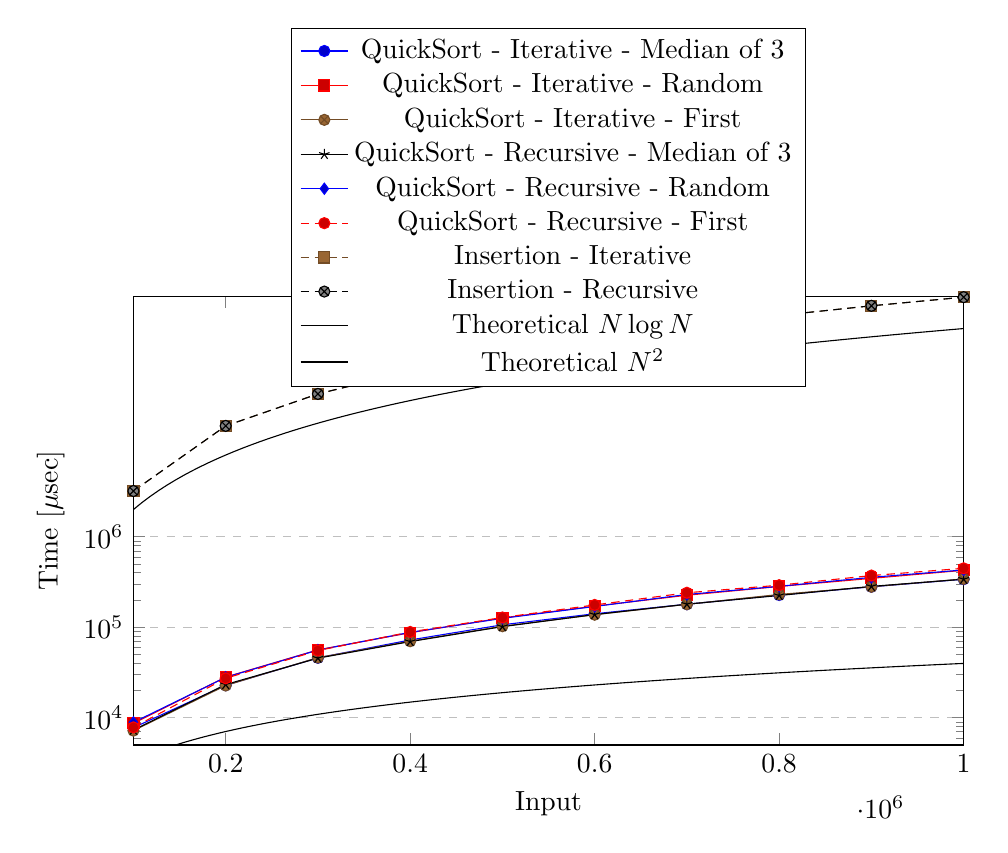
\begin{tikzpicture}
\begin{axis}[
    % title={Running times},
    width=1.0\textwidth,
    height=0.6\textwidth,
    xmode=normal,
    ymode=log,
    xlabel={Input},
    ylabel={Time [$\mu$sec]},
    xmin=100000, xmax=1000000,
    ymin=5000, ymax=450000000,
    xtick={200000, 400000, 600000, 800000, 1000000},
    ytick={10e1, 10e2, 10e3, 10e4, 10e5},
    legend style={at={(0.5,1.6)},anchor=north},
    ymajorgrids=true,
    grid style=dashed]


\addplot
    coordinates {
   (100000, 7768) (200000, 22842) (300000, 45915) (400000, 72368) (500000, 106459) (600000, 140963) (700000, 179661) (800000, 227128) (900000, 279945) (1000000, 339374)
   };
\addlegendentry{QuickSort - Iterative - Median of 3}

\addplot
    coordinates {
   (100000, 8666) (200000, 28145) (300000, 56243) (400000, 87056) (500000, 126827) (600000, 171124) (700000, 225895) (800000, 282343) (900000, 347093) (1000000, 426303)
   };
\addlegendentry{QuickSort - Iterative - Random}

\addplot
    coordinates {
   (100000, 7203) (200000, 22703) (300000, 46195) (400000, 70120) (500000, 102644) (600000, 137608) (700000, 179252) (800000, 230337) (900000, 280269) (1000000, 341778)
   };
\addlegendentry{QuickSort - Iterative - First}

\addplot
    coordinates {
   (100000, 7314) (200000, 23289) (300000, 45564) (400000, 69448) (500000, 101572) (600000, 138146) (700000, 179795) (800000, 224402) (900000, 282829) (1000000, 339602)
   };
\addlegendentry{QuickSort - Recursive - Median of 3}

\addplot
    coordinates {
   (100000, 8893) (200000, 28000) (300000, 55970) (400000, 87858) (500000, 125428) (600000, 169666) (700000, 230255) (800000, 283449) (900000, 356192) (1000000, 429718)
   };
\addlegendentry{QuickSort - Recursive - Random}

\addplot
    coordinates {
   (100000, 7829) (200000, 27278) (300000, 55275) (400000, 88720) (500000, 128185) (600000, 176467) (700000, 240455) (800000, 291557) (900000, 372641) (1000000, 448092)
   };
\addlegendentry{QuickSort - Recursive - First}

\addplot
    coordinates {
   (100000, 3206763) (200000, 16788626) (300000, 37873144) (400000, 67312389) (500000, 106012421) (600000, 154062755) (700000, 211576976) (800000, 278929902) (900000, 356658206) (1000000, 444254885)
   };
\addlegendentry{Insertion - Iterative}

\addplot
    coordinates {
   (100000, 3200947) (200000, 16792348) (300000, 37887400) (400000, 67296243) (500000, 106003174) (600000, 154032848) (700000, 211650448) (800000, 278894405) (900000, 356608103) (1000000, 444065625)
   };
\addlegendentry{Insertion - Recursive}


\addplot [
    domain=100000:1000000, 
    samples=100, 
    ]
    {x*log2(x) * 0.002};
\addlegendentry{Theoretical $N \log N$}

\addplot [
    domain=100000:1000000, 
    samples=100, 
    ]
    {x*x*0.0002};
\addlegendentry{Theoretical $N^2$}

\end{axis}
\end{tikzpicture}
\captionof{figure}{Running times of all the tested algorithms.}
\end{center}

\definecolor{RYB1}{RGB}{218,232,252}
\definecolor{RYB2}{RGB}{245,245,245}

\begin{center}
\begin{tikzpicture}
    \begin{axis}[
	    symbolic x coords={ QuickSort - Iterative - Median of 3, QuickSort - Iterative - Random, QuickSort - Iterative - First, QuickSort - Recursive - Median of 3, QuickSort - Recursive - Random, QuickSort - Recursive - First, Insertion - Iterative, Insertion - Recursive },
            % symbolic x coords={Name1, Name2, Name3},
	    xtick=data,
	    ylabel=Execution Time($\mu$ seconds),
	    ymin=0,
            xticklabel style={rotate=60,anchor=north east},
            ymajorgrids,yminorgrids,minor y tick num=4,
	    width=\linewidth
	]

            \addplot[ybar,fill=RYB1] coordinates {
		(QuickSort - Iterative - Median of 3, 339374)
		(QuickSort - Iterative - Random, 426303)
		(QuickSort - Iterative - First, 341778)
		(QuickSort - Recursive - Median of 3, 339602)
		(QuickSort - Recursive - Random, 429718)
		(QuickSort - Recursive - First, 448092)
		(Insertion - Iterative, 444254885)
		(Insertion - Recursive, 444065625)
            };

    \end{axis}
\end{tikzpicture}
    \captionof{figure}{Comparison of algorithms running with input size $10^6$.}
\end{center}

\newpage
\section{Quick Sort}
Quick sort is based on the concept of divide and conquer, it is fundamentally recursive even if it can be implemented iteratively. At each "stage" it splits the array into two and orders those parts so when the final layer of recursion is done it will be an array of 2 elements.\\
It has a worst case time complexity of $\mathcal{O}(N^2)$, this happens when the pivot splits the array into sizes of $1$ and $n - 1$. This can be avoided by picking a good pivot that represents the median of the data, theoretically if the median of each split could be known it would have a worst case time complexity of $\mathcal{O}(N\log N)$.\\
This implementation of quicksort has the optimisation of using insertion sort for smaller arrays $< 15$.

\subsection{First element pivot}

The "first pivot" method simply chooses the first element as the pivot. This approach is straightforward and easy to implement, resulting in low overhead. However, its major drawback is its sensitivity to the initial ordering of the input. If the input is already partially ordered or sorted, choosing the first element as the pivot can lead to a worst-case time complexity scenario, where the algorithm's performance degrades significantly. \\

\textbf{Computation on $T(N)$}\\
Expected complexity: $\mathcal{O}(N \log N)$\\

\[
\begin{gathered}
    T(N) = cN \log_2 N \\
    T(10^5) = 7892 = c \cdot 10^5 \cdot \log_2 10^5 \\
    c = \frac{7892}{10^5 \cdot \log_2 10^5} = 4.71 \cdot 10^{-3} \\
    T(10N) = c(10N \log_2 10N) \\
    T(10^6) = 4.71 \cdot 10^{-3}(10 \cdot 10^5 \cdot \log_2 (10 \cdot 10^5)) \approx 93947
\end{gathered}
\]

The measured value for size $10^6$ is: 448092. This is much larger and could be explained if the constants in the equation were large or if the pivot picked was bad and the solution time approached the worst case of $\mathcal{O}(N^2)$

\subsection{Median of 3 elements}

The "median of three" method attempts to make an estimated guess of the median of the array, it selects the median value among the first, middle, and last elements as the pivot. One advantage of this method is its resilience to outliers, as it reduces the likelihood of choosing a pivot that is an extreme value. This results in better performance for datasets with partially ordered elements or small variations in input distribution. However, the median of three method incurs additional comparisons to find the median, increasing the overhead for already sorted or nearly sorted arrays. \\

\textbf{Computation on $T(N)$}\\
Expected complexity: $\mathcal{O}(N \log N)$\\

\[
\begin{gathered}
    T(N) = cN \log_2 N \\
    T(10^5) = 7314 = c \cdot 10^5 \cdot \log_2 10^5 \\
    c = \frac{7314}{10^5 \cdot \log_2 10^5} = 4.40 \cdot 10^{-3} \\
    T(10N) = c(10N \log_2 10N) \\
    T(10^6) = 4.40 \cdot 10^{-3}(10 \cdot 10^5 \cdot \log_2 (10 \cdot 10^5)) \approx 87768
\end{gathered}
\]

The measured value for size $10^6$ is: 339602. This could be explained for similar reasons as the First Element Pivot.


\subsection{Random element pivot}

The "random pivot" method aims to mitigate the issues associated with deterministic pivot selection. By randomly selecting a pivot from the array, the algorithm becomes less predictable and is less likely to encounter worst-case scenarios. This method generally provides good average-case performance across a wide range of inputs. However, the randomness introduces an element of unpredictability, making it challenging to analyze and guarantee the algorithm's behavior in all cases. Additionally, the overhead of generating random numbers may impact performance, especially for large datasets. \\

\textbf{Computation on $T(N)$}\\
Expected complexity: $\mathcal{O}(N \log N)$\\

\[
\begin{gathered}
    T(N) = cN \log_2 N \\
    T(10^5) = 8893 = c \cdot 10^5 \cdot \log_2 10^5 \\
    c = \frac{8893}{10^5 \cdot \log_2 10^5} = 5.35 \cdot 10^{-3} \\
    T(10N) = c(10N \log_2 10N) \\
    T(10^6) = 5.35 \cdot 10^{-3}(10 \cdot 10^5 \cdot \log_2 (10 \cdot 10^5)) \approx 106715
\end{gathered}
\]

The measured value for size $10^6$ is: 429718. This could be explained for similar reasons as the First Element Pivot.

\newpage
\section{Insertion Sort}

Insertion sort's efficiency stands out when handling small or partially ordered datasets. It is perfectly suited for applications were the whole data set for sorting isn't available at once, it can be fed more data to sort without having to start it operating over.However, it faces faces limitations with larger or randomly ordered datasets, as its quadratic time complexity $\mathcal{O}(N^2)$ becomes a bottleneck. The need for frequent comparisons and element shifts makes it less efficient compared to more advanced sorting algorithms for extensive datasets. \\

\textbf{Computation on T(N)}\\

Expected complexity: $O(N^2)$\\

\[
\begin{gathered}
    T(N) = cN^2 \\
    T(10^5) = 3200947 = c \cdot 10^5 \cdot \log_2 10^5 \\
    c = \frac{3200947}{10^5 \cdot \log_2 10^5} = 3.20 \cdot 10^{-4} \\
    T(10N) = c(10N)^2 \\
    T(10^6) = 5.35 \cdot 10^{-3}(10^6)^2 \approx 320094700
\end{gathered}
\]

The measured value for $10^6$ is: 444065625 which is close to the theoretical value. It is expected that insertion was the slowest of the algorithm as it was not suited to the data it was given. 

\newpage

\newpage
\section{Binary Search}


\begin{center}
\begin{tikzpicture}
\begin{axis}[
    %title={Running times},
    width=1.0\textwidth,
    height=0.6\textwidth,
    xmode=normal,
    ymode=normal,
    xlabel={Input},
    ylabel={Time [msec]},
    xmin=200000, xmax=1000000,
    ymin=0, ymax=158,
    xtick={200000, 400000, 600000, 800000, 1000000},
    ytick={},
    legend pos=north west,
    ymajorgrids=true,
    grid style=dashed,
    legend pos=north west]
\addplot
    coordinates {
	(100000, 25) (200000, 82) (300000, 106) (400000, 151) (500000, 230) (600000, 180) (700000, 228) (800000, 174) (900000, 158) (1000000, 158)
    };
\addlegendentry{Binary Search}
\end{axis}
\end{tikzpicture}
\captionof{figure}{Running times of Binary Search.}
\end{center}

Binary search is a highly efficient algorithm used for finding a specific element in a sorted array. One of its main advantages is its speed, as it has a logarithmic time complexity of $\mathcal{O}(\log N)$. It works by continually splitting the array into 2 parts until it finds the target element. The only limitation binary search is that it requires that the array be sorted. \\

\textbf{Computation on T(N)}\\

Expected complexity: $O(logN)$\\

\[
\begin{gathered}
    T(N) = c\log_2 N \\
    T(10^5) = 25 = c \cdot 10^5 \cdot \log_2 10^5 \\
    c = \frac{25}{\log_2 10^5} = 2.50 \cdot 10^{-9} \\
    T(10N) = c(\log_2 10N) \\
    T(10^6) = 2.50 \cdot 10^{-9}(\log_2 (10 \cdot 10^5)) \approx 2500
\end{gathered}
\]

\textbf{Analysis}\\

Binary search is so fast that it is difficult to time it accurately, hundreds of runs of binary sort over an input size of $10^6$ resulted in average times (over 10 runs) ranging from 5 to 200 $\mu$sec. It was not possible to run for a size than $10^6$ due to the restriction of having to implement it recursively and running out of stack space. 

\newpage
\section{Conclusion}

Sorting algorithms play a crucial role in various applications due to their significance, utility, and widespread usage. Identifying the most efficient algorithm for a specific application can result in significant advantages. However, the alignment between theoretical analysis and practical implementation is not always guaranteed. Therefore, it becomes imperative to thoroughly test the chosen algorithm before making a definitive decision. The unique use case and the selected data structures can profoundly influence the ultimate efficiency, distinguishing a successful implementation from an unsuccessful one.

\newpage

\nocite{*}
\printbibliography[] % to hide showing references again

\end{document}
